%%%%%%%%%%%%%%%%%%%%%%%%%%%%%%%%%%%%%%%%%
% Journal Article
% LaTeX Template
% Version 1.3 (9/9/13)
%
% This template has been downloaded from:
% http://www.LaTeXTemplates.com
%
% Original author:
% Frits Wenneker (http://www.howtotex.com)
%
% License:
% CC BY-NC-SA 2.5 (http://creativecommons.org/licenses/by-nc-sa/3.0/)
%
%%%%%%%%%%%%%%%%%%%%%%%%%%%%%%%%%%%%%%%%%

%----------------------------------------------------------------------------------------
%	PACKAGES AND OTHER DOCUMENT CONFIGURATIONS
%----------------------------------------------------------------------------------------

\documentclass[twoside]{article}
\usepackage{datetime}
\usepackage{stackengine}
\usepackage{mathtools}
\usepackage{graphicx}
\renewcommand\useanchorwidth{T}
\usepackage{xcolor}
\def\theyearwidth{1.5pt}
\def\mystrut{\rule{0ex}{.1ex}}
\def\myyrstrut{\rule[-1ex]{0ex}{2ex}}
\newlength\yrsfboxrule
\yrsfboxrule .4\fboxrule
\newcommand\yearwidth[1]{\def\theyearwidth{#1}\ignorespaces}
\newcommand\skipyears[2][black]{%
  \fboxrule\yrsfboxrule%
  \fboxsep=-\yrsfboxrule%
  \fcolorbox{#1}{#1}{\mystrut\hspace{#2}}%
  \ignorespaces%
}
\newcommand\showyear[2][black]{%
  \fboxsep=0pt%
  \stackunder[2pt]{%
    \colorbox{#1}{\myyrstrut\hspace{\theyearwidth}}%
  }{\tiny#2}%
  \ignorespaces%
}
\usepackage{lipsum} % Package to generate dummy text throughout this template

\usepackage[sc]{mathpazo} % Use the Palatino font
\usepackage[T1]{fontenc} % Use 8-bit encoding that has 256 glyphs
\linespread{1.05} % Line spacing - Palatino needs more space between lines
\usepackage{microtype} % Slightly tweak font spacing for aesthetics

\usepackage[hmarginratio=1:1,top=32mm,columnsep=20pt]{geometry} % Document margins
\usepackage{multicol} % Used for the two-column layout of the document
\usepackage[hang, small,labelfont=bf,up,textfont=it,up]{caption} % Custom captions under/above floats in tables or figures
\usepackage{booktabs} % Horizontal rules in tables
\usepackage{float} % Required for tables and figures in the multi-column environment - they need to be placed in specific locations with the [H] (e.g. \begin{table}[H])
\usepackage{hyperref} % For hyperlinks in the PDF

\usepackage{lettrine} % The lettrine is the first enlarged letter at the beginning of the text
\usepackage{paralist} % Used for the compactitem environment which makes bullet points with less space between them

\usepackage{abstract} % Allows abstract customization
\renewcommand{\abstractnamefont}{\normalfont\bfseries} % Set the "Abstract" text to bold
\renewcommand{\abstracttextfont}{\normalfont\small\itshape} % Set the abstract itself to small italic text

\usepackage{titlesec} % Allows customization of titles
\renewcommand\thesection{\Roman{section}} % Roman numerals for the sections
\renewcommand\thesubsection{\Roman{subsection}} % Roman numerals for subsections
\titleformat{\section}[block]{\large\scshape\centering}{\thesection.}{1em}{} % Change the look of the section titles
\titleformat{\textbf}[block]{\large}{\thesubsection.}{1em}{} % Change the look of the section titles

\usepackage{fancyhdr} % Headers and footers
\pagestyle{fancy} % All pages have headers and footers
\fancyhead{} % Blank out the default header
\fancyfoot{} % Blank out the default footer
\fancyhead[C]{Approximation Algorithms for Stochastic Inventory Control Models $\bullet$ \ddmmyyyydate\today } % Custom header text
\fancyfoot[RO,LE]{\thepage} % Custom footer text


%----------------------------------------------------------------------------------------
%	TITLE SECTION
%----------------------------------------------------------------------------------------

\title{\vspace{-15mm}\fontsize{24pt}{10pt}\selectfont\textbf{Approximation Algorithms for Stochastic Inventory Control Models}}\vspace{-6ex} % Article title
\author{Hao Yuan
\and
Feng Wei
\and
Blake Miller
}
\date{}
%----------------------------------------------------------------------------------------

\begin{document}

\maketitle\vspace{-6ex} % Insert title
\thispagestyle{fancy} % All pages have headers and footers

%----------------------------------------------------------------------------------------
%	ABSTRACT
%----------------------------------------------------------------------------------------

%\begin{abstract}%

%\noindent \lipsum[1] % Dummy abstract text%

%\end{abstract}
\begin{center}
{\ttfamily Github:\href{https://github.com/blakeapm/stochastic-inventory}{github.com/blakeapm/stochastic-inventory}}
\end{center}\vspace{-2ex}

%----------------------------------------------------------------------------------------
%	ARTICLE CONTENTS
%----------------------------------------------------------------------------------------

\begin{multicols}{2} % Two-column layout throughout the main article text

\section{Introduction}

\lettrine[nindent=0em,lines=2]{P}roper inventory management, stocking, and purchasing policy are paramount to supply, distribution, and retail businesses. The challenges of minimizing costs in an environment dependent upon many stochastic processes presents businesses with a unique challenge. This problem is important for any company that seeks to minimize cost of holding excess inventory while minimizing backorder costs (unmet demand). Especially in industries where the demand environment is highly dynamic. (i.e. Apple's supply-chain for solid state drives, seasonal products such as rock salt). \\
The inventory control problem is very difficult because oftentimes demand are unpredictable and cost is hard to predict due to the nature of demand. It is even very difficult to develop an approximation algorithm that is appropriate to the risk profile of companies operating under dynamic demand environments. This is because these companies must determine whether the provable error margin of an approximation algorithm is appropriate for their own risk profile. In this paper, we will investigate the performance a new algorithm\cite{CLAcha2} for the inventory control problem using C++ implementation.\\

%------------------------------------------------

\section{The Model}
    First, let's look at a simplied model with leading time $L=0$, i.e. the product arrive immediatelly after ordering. Then, we consider finite time horizon $T$:
    \par
      {\centering\yearwidth{1pt}\tclap{\tiny t}\showyear{1}\skipyears[black]{.25in}\showyear{2}\skipyears[black]{.25in}\showyear{3}\skipyears[black]{.25in}\showyear{4}\skipyears[black]{.25in}\showyear{5}\skipyears[black]{.25in}\showyear{6}\skipyears[black]{.25in}$\text{  }\cdots\text{  }$\showyear{$T-1$}\skipyears[black]{.25in}\showyear{$T$}
    \par}
    \vspace{0.1in}
    At each time period $t \in \{1,\cdots,T\}$, the following cost are incurred:
    \begin{equation}\label{eq:Ldef}
    \begin{array}{rl}
        & L_t(x_t,d_t,q_t)\\
        := & c_tq_t + h_t(x_t + q_t - d_t)^{+}+p_t(x_t + q_t -d_t)_{t}^{-}
    \end{array}
    \end{equation}
        where
    \begin{compactitem}
      \item $c_t$: per-unit ordering cost.
      \item $h_t$: per-unit holding cost.
      \item $p_t$: per-unit backlogging penalty.
      \item $x_t$: net inventory (state).
      \item $q_t$: ordering quantity (control).
      \item $d_t$: demand quantity (we observe $d_t$ after decide $q_t$).
    \end{compactitem}

    In Eq. (\ref{eq:Ldef}), $x_t + q_t - d_t$ is the net inventory at the end of period $t$, if it is positive, we will suffer from a holding cost $h_t(x_t + q_t - d_t)^{+}$, otherwise there will be backlogging cost $p_t(x_t + q_t - d_t)^{-}$. Together with the ordering cost $c_tq_t$, we define $L_t(x_t,d_t,q_t)$ to be our Local Cost at time $t$, i.e. Local Cost = Ordering Cost + Holding Cost + Backlogging Cost.\\
    Our goal is at each time $t$, choose $q_t$ to minimize the expected total cost from period $t$ to $T$. To do this we will find out the minimizer $q_t$ (or approximate minimizer) of the quantities below:
    \begin{equation}\label{eq:Vt}
    \begin{array}{rl}
    & V_T(x_T,d_{1..T-1}) \\
    = & \min_{q_T \geq 0} E[L_T(x_T,D_T,q_T) | d_{1..T-1}]\\
    &V_t(x_t,d_{1..t-1}) \\
    = & \min_{q_t \geq 0} E[L_t(x_t,D_t,q_t)\\
    & +V_{t+1}(x_t + q_t - D_t, d_{1..t-1},D_t)|d_{1..t-1}]
    \end{array}
    \end{equation}
    where $V_t$ is the minimum expected cost from period $t$ to $T$, $d_{t_1..t_2}$ is the demand vector from $t_1$ to $t_2$. Since at time $t$, the future demand are some random variables depending on previous demand, we use $D_t$ to denote those unknow demand. Then, this gives us two natural ways to "solve" the problem:
    \begin{compactitem}
      \item
        Dynamic Programming: solve for $q_t$ backwards using the formula above.
      \item
        Myopic: At time $t$, ignore $V_{t+1}$, we only minimize $E[L_t(x_t,D_t,q_t)|d_{1..t-1}]$.
    \end{compactitem}
     However, using dynamic programming, at period $s>t$, $D_s$ is a random variable that depends on perivous demands $d_1, d_2,...,d_{t+1},...,d_{s-1}$ which lead to computational difficulties. We also need to work on $q_t,...,q_T$ which are our unknown future decision. Both of above make dynamic programming intractable. On the other side, although myopic approach works extremely well on many cases\cite{CLAcha1}, it may perform extremely poorly on some cases, which will be shown at the end of the paper.\\

    In fact we also need to consider leading time $L \neq 0$, i.e. it takes $L$ periods to receive our order. Then we need define $x_t={\rm Net~Inventory}  + \sum_{j = t - L+1}^{t-1} q_j$ to be our inventory position, where $\sum_{j = t - L+1}^{t-1} q_j$ is our undelivered orders. We also need to modify our Local Cost to be 
        \begin{equation}\label{eq:Lneq0}
        \begin{array}{rl}
              & L_t(x_t,d_{t..t+L},q_t)\\
          := &c_tq_t + h_{t+L}(x_t + q_t - d_{[t,t+L]})^{+}\\
                                &  + p_{t+L}(x_t + q_T - d_{[t,t+L]})^{-}
        \end{array}
        \end{equation}
        where $d_{[t,t+L]}=\sum_{s=t}^{t+L} d_s$.\\
        In the simulation, we can always assume $c_t = 0$ by doing the transformation ($c_{T+1}:=0$):
        \begin{equation}\label{eq:hats}
        \begin{array}{rl}
          \hat{h_t} &:= h_t + c_t - c_{t+1}\\
          \hat{p_t} &:= p_t - c_t + c_{t+1}\\
        \end{array}
        \end{equation}

\section{Dual Balancing Algorithm}    
    In 2007, R. Levi, M. Pal, R. Roundy and D. Shmoys introduced a new approach\cite{CLAcha2} for the inventory control problem named Dual Balancing. Recall Local Backlogging Cost:
    \begin{equation}\label{eq:Bcost}
    \Pi_t(x_t,q_t) = p_{t+L}(x_t + q_T - D_{[t,t+L]})^{-}
    \end{equation}
    Now, we define Marginal Holding Cost:
    \begin{equation}\label{eq:MHcost}
    H_t(x_t,q_t) := \sum_{j = t+L}^{T} h_j (q_t - (D_{[t,j]} - x_t)^+)^+.
    \end{equation}
    Now, the Dual Balancing Algorithm as follows:\\
    (i) Transform using Eq. (\ref{eq:hats});\\
    (ii) Start at $t=1$;\\
    (iii) Solve the convex optimization problem:
    \begin{equation}\label{eq:ConvexOP}
        \min_{q_t > 0}\\ \max{E[H_t(x_t,q_t)| d_{1..t-1}], E[\Pi_t(x_t,q_t)| d_{1..t-1}]};
        \end{equation}
    (iv) Observe $d_t$, update $x_t,d_{1..t}$ and set $t=t+1$;
    (v) If $t<T$, go to step (iii).\\

    In fact, the above algorithm is called Dual Balancing since the minimizer $q_t$ in Eq. (\ref{eq:ConvexOP})will satisfy
    \begin{equation}\label{eq:DB}
        E[H_t(x_t,q_t)| d_{1..t-1}] = E[\Pi_t(x_t,q_t)| d_{1..t-1}]
        \end{equation}
      Since both $H_t,\Pi_t$ don't depend on $q_s$ for $s>t$, the Dual-Balancing algorithm can be computed online, i.e. we can compute $q_t$ without compute $q_{t+1}, q_{t+2} ... $. It was proven that, the expected total cost in Dual-Balancing algorithm,  is at most two times the optimal one\cite{CLAcha2}.
% \lipsum[4] % Dummy text

%------------------------------------------------

\section{Implementation}

%\begin{figure}[htb]
%\centering
%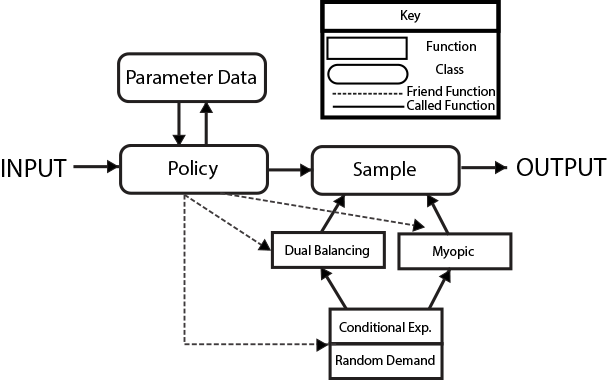
\includegraphics[scale=0.5,bb=0 0 385 567]{software_diagram.png}
%\caption{GENERALIZED}
%\label{fig:implementation}
%\end{figure}

\begin{center}
  \label{figure:software_diagram}
  \captionof{figure}{Software Design Diagram}
  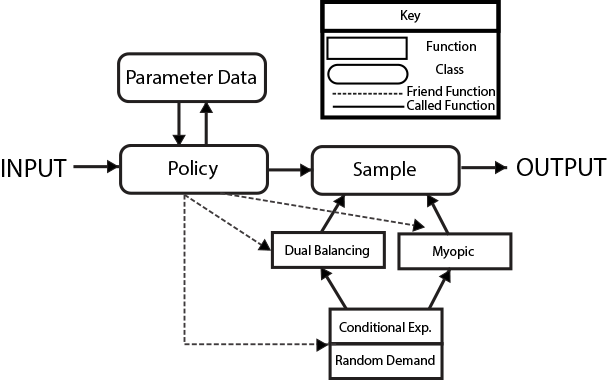
\includegraphics[width=3.0in]{software_diagram.png}
\end{center}
Our aim is to implement Dual Balancing Algorithm and test its performance for some common demand distributions. We divide coding into several major parts. The Parameter Data class save parameters for the problem, while its child class Policy contains all the informations for the algorithm, including, demand distribution type, distribution parameter, demand, ordering and cost for all time periods, and so on. Class Sample is in charge of organizing all functions, classes and collecting data.\\
Once read data from input file, the program contruct a Sample class for each data set, the Sample class will construct a Policy class and updating the Policy class as the algorithm is called. We provide both Dual Balancing and Myopic for comparison. The main challenge is to compute those conditional expectation in Eq. (\ref{eq:Bcost})(\ref{eq:MHcost})(\ref{eq:DB})) using the function ConditionalExp for some given distribution. Once get the conditional expectations, we solve the minimization problem at current time $t$, then we receive a random demand from RandomDemand and move on. After all computation is finished, the Sample class will collect the data and provide the output.



\section{Results}

In simulations, we have following default setting without special mentioning:
\begin{compactitem}
      \item $c_t = 3, h_t = 1, p_t = 2, L=5, x_0=0$.
      \item The sample size are 20.
      \item We considered four different demands (i.e. $D_t$) distribution:\\
            1. $D_t = N(50,5)$ are iid.\\
            2. $D_t-D_{t-1} = N(5,1.581)$ with $D_0=30$.\\
            3. $D_t-D_{t-1} = B(10,0.5)$ with $D_0=30$.\\
            4. $D_t- (D_{t-1} + D_{t-2} + D_{t-3})/3 = N(5,1.581)$ with $D_0=30$.
\end{compactitem}
\begin{center}
  \textbf{Single Sample Path Behavior}
\end{center}
\begin{center}
  \label{figure:DualBalancingParameters}
  \captionof{figure}{Dual Balancing Parameters}
  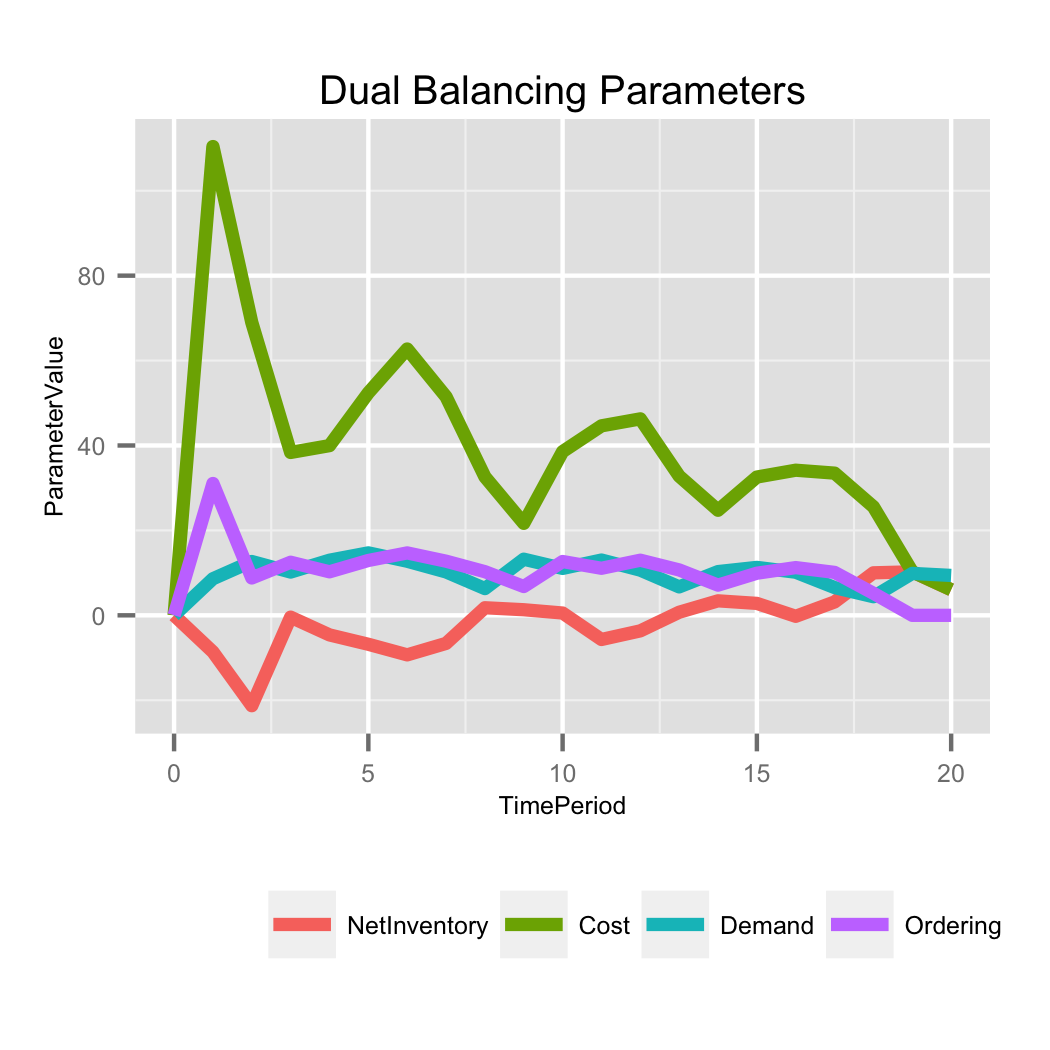
\includegraphics[width=2.5in]{figures/DualBalancingParameters.png}
\end{center}

We pick $T=20,L=2,D_t=N(20,2,24)$ i.i.d. and compute using Dual Balancing. In the Fig. \ref{figure:DualBalancingParameters}, we only show the result of one sample path. Since the initial net inventory is 0 and $L=2$, the demand is going to accumulate and induce a nonzero holding cost. However, due to a large amount of ordering at beginning, the cost reduced a lot when the first ordering arrived at $t=L=2$. After that, the ordering stabilized and oscillate according to the change of $d_t$. The net inventory\footnote{Net inventory is computed by averaging absolute value of net inventory in each sample. Small net inventory indicates good police.} is also stabilize and oscillate around 0. This means the holding cost and backlogging cost are close to zero. Most of the cost are due to ordering and the cost curve is almost proportional to demand one.\\
Since, the demand include randomness, we will never be able to control our net inventory exactly at zero. Thus, Fig. \ref{figure:DualBalancingParameters} actually imply that the solution of Dual Balancing could be very close to the optimal solution.
\begin{center}
  \textbf{Average Behavior}
\end{center}

\begin{center}
  \label{figure:NetInventoryLeadTime}
  \captionof{figure}{\small Stabilization Across Different Initial Values of Net Inventory and Lead Time}
  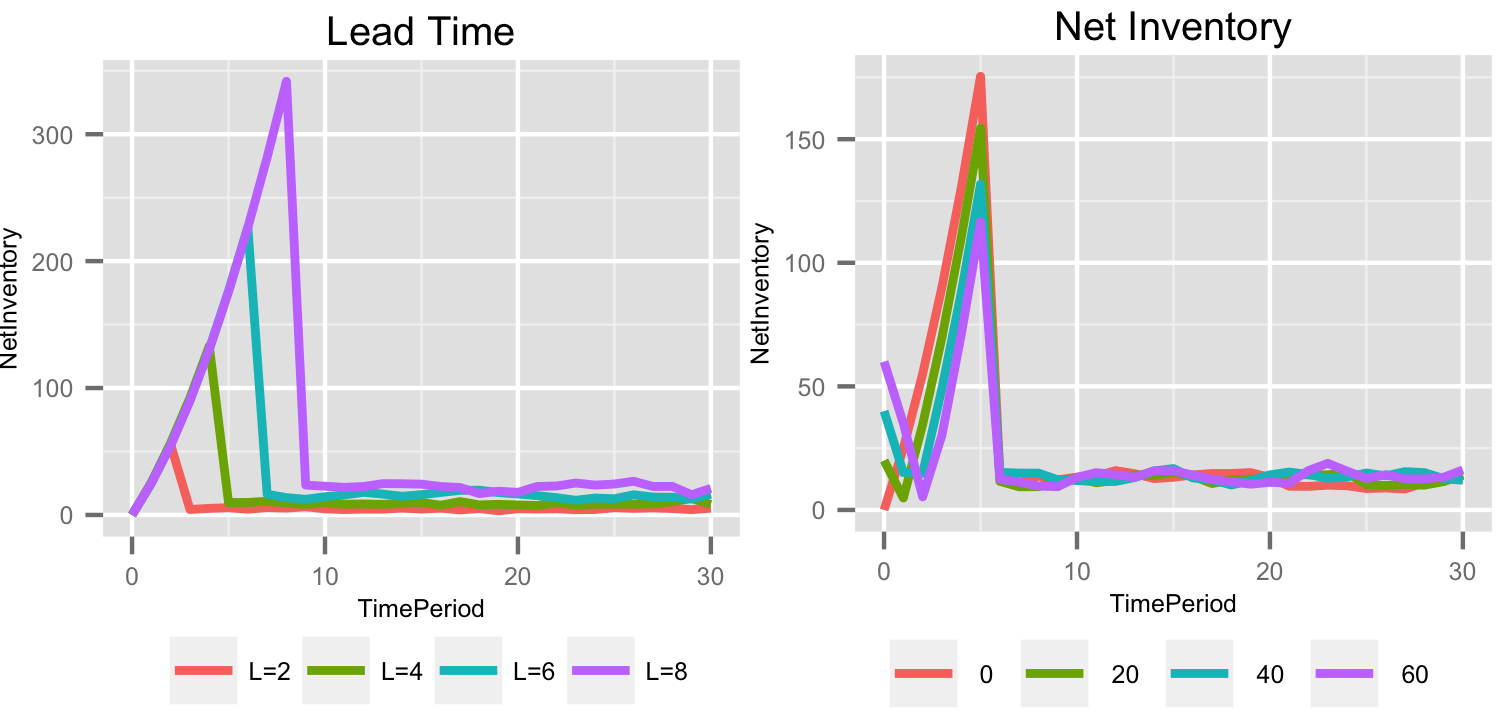
\includegraphics[width=2.8in]{figures/NetInventoryLeadTime.png}
\end{center}

In Fig. \ref{figure:NetInventoryLeadTime}, we fix $T=30,D_t-D_{t-1} = N(5,1.581)$ with $D_0=20$ and using Dual Balancing algorithm. These two plots show us some nice convergence behaviors. In the left figure, we choose initial inventory $x_0 = 0$ and plot net inventory for different leading times. In the left plot, we see no matter how larger our leading that is, at period $L+1$, i.e. the time we receive our period 1 order, the net inventory drop down a low level immediately. Although all net inventory are close to zero in long run, the larger leading time still leads to a slightly higher volume of net inventory. In the right figure, a fix $L = 5$ and change initial net inventory. If initial net inventory $x > 0$, it will support demands for some periods, and after consuming all initial net inventory, the absolute net inventory climbs up. However at $t=L=1$ we always have a stable net inventory closed to 0. And we can see the stabilized net inventory won't depend on $x_0$.\\

\begin{center}
  \textbf{Long Term Cost/Demand Ratio}
\end{center}
\begin{center}
  \label{figure:TotalCostToOrderRatio}
  \captionof{figure}{Total Cost to Order Ratio: Independent Normal vs. Incrementing Normal Distribution}
  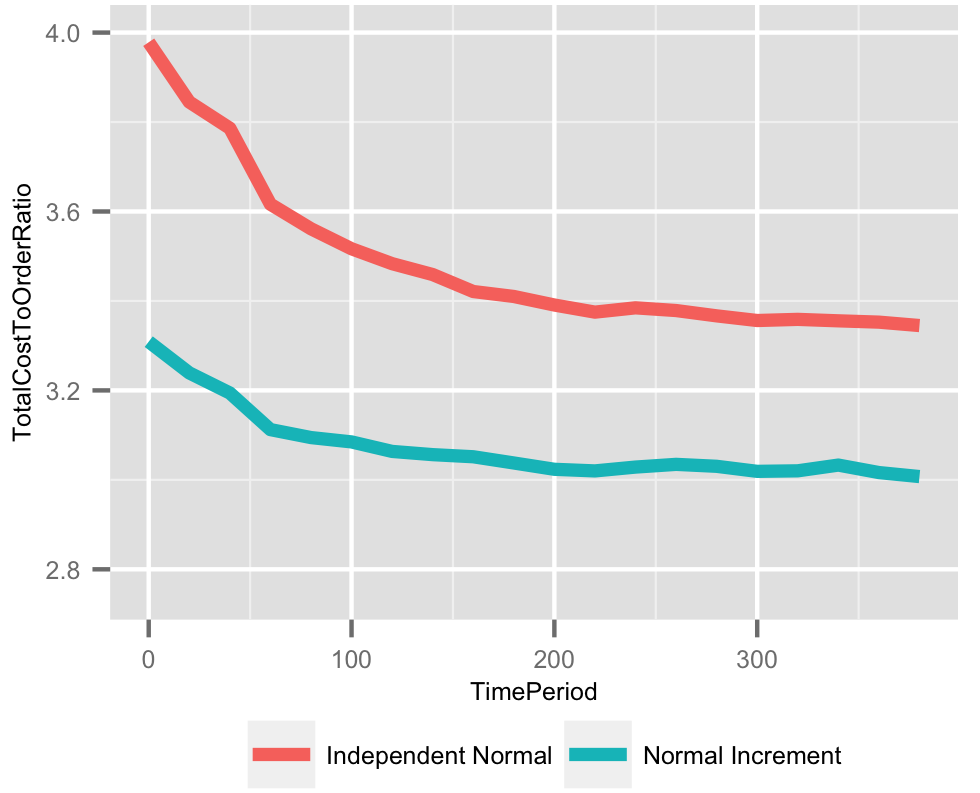
\includegraphics[width=2.8in]{figures/TotalCostToOrderRatio.png}
\end{center}
Another thing we interested in is whether Dual Balancing still perform very well as $T$ getting large. In Fig. \ref{figure:TotalCostToOrderRatio}, both curves plotted total cost over total demand for different distributions. We can see that, in the long run, the cost per demand converge to a center number and will not blow up. This imply in long run, the algorithm produced nice stability. Moreover, since our $c_t=3$, this ratio is at least 3, and you may see for normal increment, the ratio converge to exactly 3, so the Dual Balancing is almost optimal. 

\section{Comparison to Myopic}

\begin{center}
  \textbf{General Performance}
\end{center}

\begin{center}
  \captionof{figure}{\scriptsize Accumulative Demand and Accumulative Cost}
  \label{figure:AccumulativeDemandAndCost}
  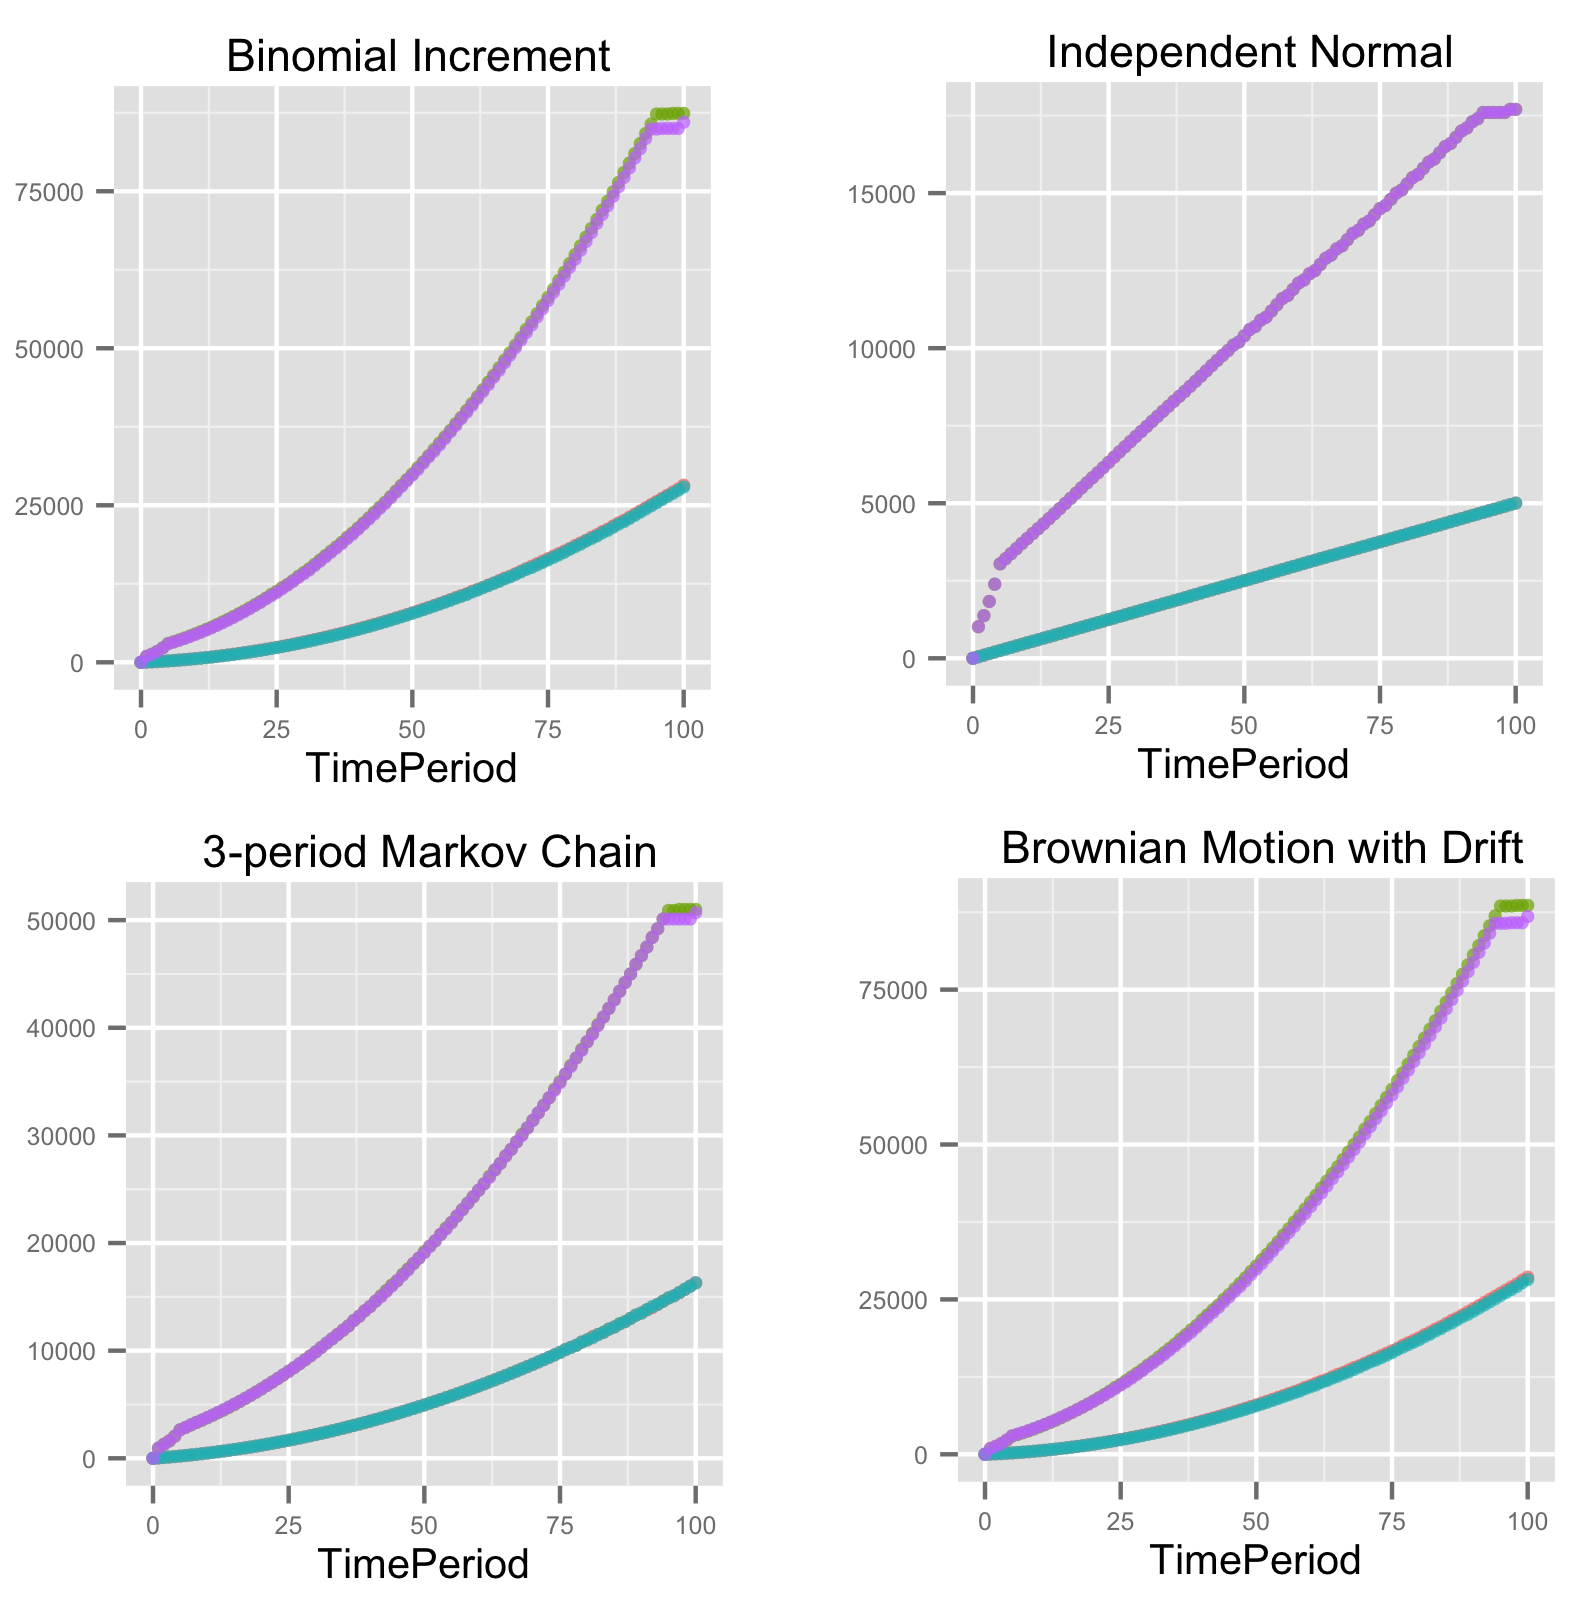
\includegraphics[width=2.8in]{figures/AccumulativeDemandAndCost.png}
  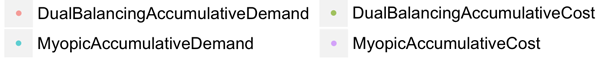
\includegraphics[width=2.8in]{figures/key.png}
\end{center}

In Fig. \ref{figure:AccumulativeDemandAndCost}, we compare the averaged sample pathes of the two appraoches. We notice that for all four kinds for demand distributions, the accumulative demands for both algorithm overlap on the green line and accumulative costs overlap on the purple line. This indicates that for all four kinds for demand distributions, under same demands distribution, the performance, measured by accumulative cost, of Dual Balancing and Myopic are almost exactly the same. In was shown earlier\cite{CLAcha1} that, in many cases, myopic algorithm works extremely well. Thus, Fig. \ref{figure:AccumulativeDemandAndCost} indicates a good performance of Dual Balancing algorithm.

  \begin{center}
    \textbf{Bad Example for Myopic}
  \end{center}
  \begin{center}
    \label{figure:MyopicBad}
    \captionof{figure}{\scriptsize Myopic vs. Dual-Balancing}
    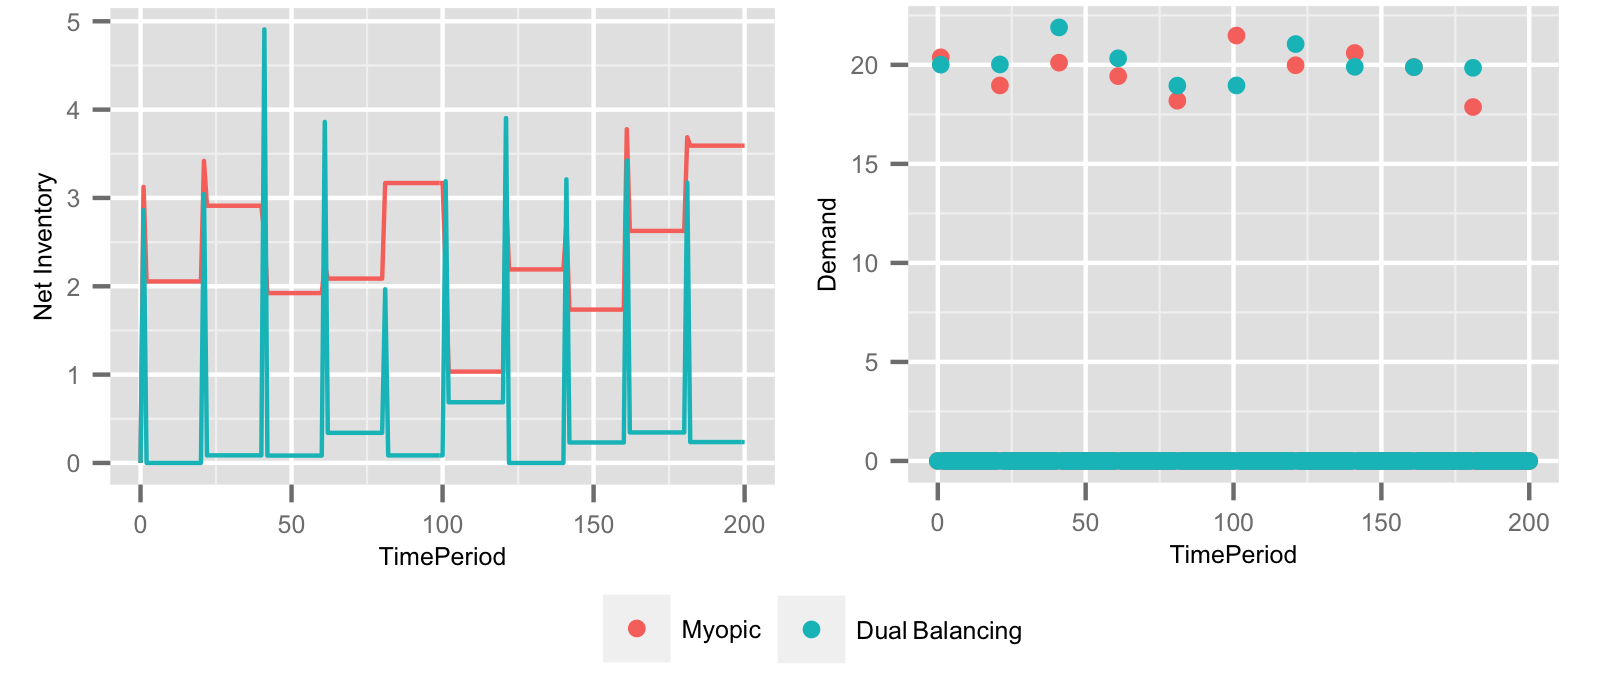
\includegraphics[width=2.8in]{figures/MyopicBad.png}
  \end{center}
  In all following figures, we averaged the sample paths. As shown in Fig. \ref{figure:MyopicBad}, We consider the a periodic demand distribution: if $t\in \{0,20,40,60,...\}$, $D_t=N(20,3.16)$, otherwise, $D_t=0$.  In Fig. \ref{figure:MyopicBad}, we can see that at critical periods (i.e. $t\in \{0,20,40,60,...\}$), net inventory have a sudden jump for for both algorithms, but after the jump the net inventory produced by applying Dual Balancing drops down to a much low level than Myopic.
  \begin{center}
    \label{figure:MyopicBadOrderingWriteup}
    \captionof{figure}{\scriptsize Myopic vs. Dual-Balancing: Ordering}
    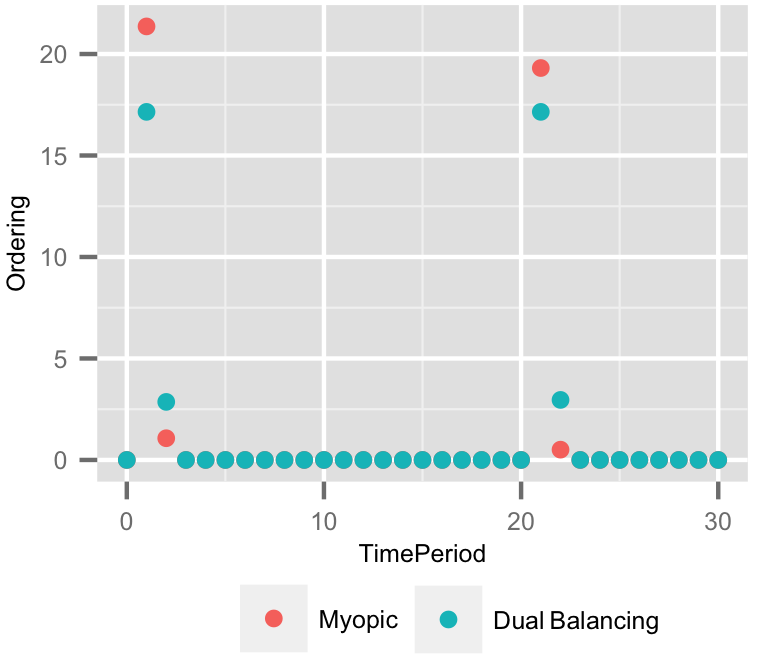
\includegraphics[width=2.5in]{figures/MyopicBadOrderingWriteup.png}
  \end{center}
  Fig \ref{figure:MyopicBadOrderingWriteup} explains why Dual Balancing algorithm has this better performance. Comparing to Myopic, Dual Balancing algorithm always orders less than Myopic algorithm on each critical period, which gives a slightly higher expected backlogging cost on this critical period, but it successfully avoided possible holding cost during all the periods before next demand arrived 20 days later as we see in Fig. \ref{figure:MyopicBadOrderingWriteup}. Then in next period, dual balancing ordered a little bit to eliminate the backlogging cost. Then in following 18 periods, its cost is almost 0.

  \begin{center}
    \label{figure:MyopicBadAccumulativeCostWriteup}
    \captionof{figure}{\scriptsize Myopic vs. Dual-Balancing: Accumulative Cost}
    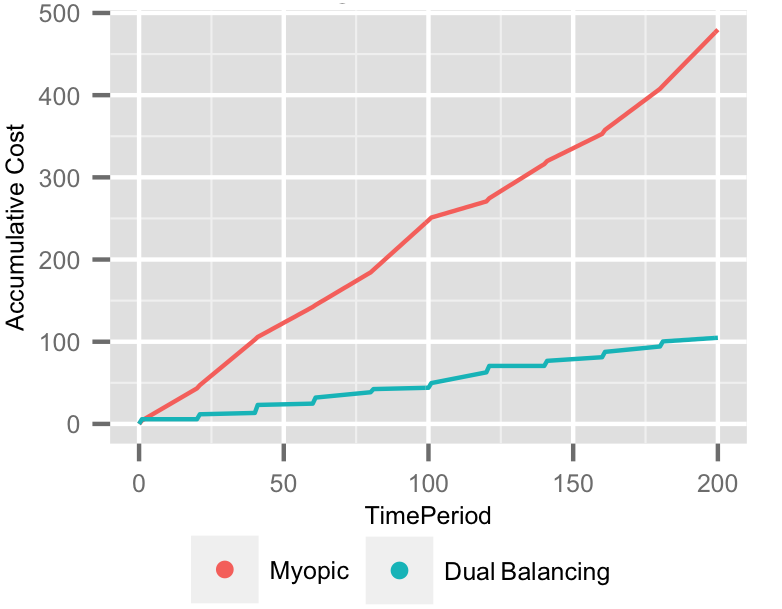
\includegraphics[width=2.5in]{figures/MyopicBadAccumulativeCostWriteup.png}
  \end{center}
  As a result of the nice strategy, Fig. \ref{figure:MyopicBadAccumulativeCostWriteup} tells us that in this case, the Myopic is about 5 times the total cost of Dual Balancing in the long run. In fact, it could be prove that the Myopic could be $K$ times the optimal cost where $K$ is the period of demand.
  %------------------------------------------------

\section{Conclusion}

In this paper, we have shown that, the Dual Balancing algorithm present very nice behavior, like converge to equilibrium very quickly, solution is almost optimal, very stable as $T$ increase and so on. The Dual Balancing performs as good as Myopic for all the cases tried, especially, for rapid change periodical demand, Dual Balancing performs much better then Myopic.\\
There are some other interesting problems about implementation in this area to be work on, like simulate dynamic programming and compare the performance to Dual Balancing, simulate continuous time control problem.

\section{Contributions}
In our Project, Hao and Feng did most of the C++ coding job, while Blake did the R coding part. Hao is the one who introduced us this interesting problem and organized meetings. Feng structured the C++ code and collected all the data. All the nice figures in this paper are work of Blake, he also provided very strong technical support in latex.

%\lipsum[7] % Dummy text

%----------------------------------------------------------------------------------------
%	REFERENCE LIST
%----------------------------------------------------------------------------------------

\begin{thebibliography}{99} % Bibliography - this is intentionally simple in this template

\bibitem{CLAcha1}
Iida, T., P. H. Zipkin. 2006. Approximate solutions of a dynamic forecast-inventory model. Manufacturing Service Oper. Management
8 407-425.
\bibitem{CLAcha2}
Retsef Levi, Martin Pal, Robin Roundy and David Shmoys, 2007. Approximation Algorithms for Stochastic Inventory Control Models, Mathematics of Operations Research, Volume 32 (2), pages 284-302.

\end{thebibliography}

%----------------------------------------------------------------------------------------

\end{multicols}

\end{document}
